\chapter{Herramientas}
\label{chap:herramientas}
En este capítulo se van a detallar las herramientas y tecnologías utilizadas en el desarrollo de este proyecto principalmente en el ámbito web. Algunas se han elegido por facilidad de uso y otras por necesidad del entorno desarrollado.

\section{Lego Ev3}
\label{sec:caracteristicas} 
Dentro de los robots de \textit{LEGO} el que mas versatilidad, además de más potencia de procesamiento y posibilidades en las opciones de creatividad a la hora de crear robots es \textit{LEGO MINDSTORMS Education}(Pack en el que viene integrado el \textit{LEGO Ev3}) tambien trae una mayor gama de sensores, por no decir que es uno de los lideres en la educación STEM (siglas en inglés de Ciencias, Tecnología,Ingeniería y Matemática), En el centro de \textit{LEGO MINDSTORMS Education} se encuentra el Bloque EV3, el bloque inteligente programable que controla motores y sensores y además proporciona comunicación inalámbrica como quiera que sea.
 \begin{figure}[H]
    \centering
    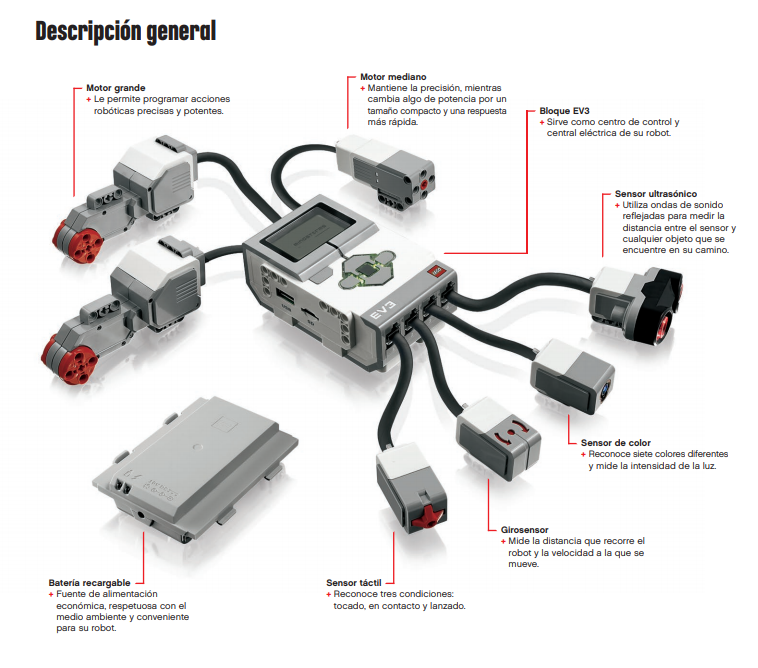
\includegraphics[scale=0.7]{img/partes.png}
    \caption{Conjunto Ev3} \label{fig:partes}
\end{figure}
 Esto quiere decir que las posibilidades a la hora de crear diferentes robots, con diferentes configuraciones de sensores, son prácticamente infinitas. Pero vamos a centrarnos en los casos que mas funcionalidad tienen. El robot que mas versatilidad presenta a la hora de superar ejercicios, es un robot triciclo, con dos ruedas delanteras y una pivotante trasera. Así que este será nuestro modelo para el robot. Y ademas como el \textit{kit de LEGO MINDSTORMS} viene con tres sensores diferentes, crearé tres modelos para integrarlos por separado en la plataforma.

\section{Python}

Python es un lenguaje de programación administrado por la Python Software Foundation.Posee una licencia de código abierto, denominada Python Software Foundation License.Es un lenguaje interpretado, por lo que no se necesita compilar el código fuente para poder ejecutarlo. Esto ofrece ventajas como la rapidez de desarrollo e inconvenientes como una me-nor velocidad. En ciertos casos, cuando se ejecuta por primera vez un código, se producen unos bytecodes que se guardan en el sistema y que sirven para acelerar la compilación implícita que realiza el intérprete cada vez que se ejecuta el mismo código.Lenguaje muy popular en los últimos años gracias a la cantidad de librerías que contiene,tipos de datos y funciones incorporadas en el propio lenguaje, que ayudan a realizar muchas tareas habituales sin necesidad de tener que programarlas desde cero. Ademas, su filosofía hace hincapié en una sintaxis que favorezca un código legible, facilitando su aprendizaje.
Este lenguaje nos es muy importante en este proyecto ya que es el lenguaje nativo del robot y en el que van a ir programados los \textit{drivers} para el robot real. 

\section{HTML}

HTML (HyperText Markup Languaje) fue desarrollado en 1991 por Tim Berners-Lee mientras trabajaba en la Organización Europea para la Investigación Nuclear (CERN), y popularizado por el navegador Mosaic desarrollado en NCSA (Raggett, Le Hors y Jacobs, 1999).

Es un lenguaje de marcado que sirve para estructurar una página Web. Permite poner etiquetas a diferentes partes de la página para darles la misma apariencia. También tiene tipos de funciones para personalizar el tipo de letra y la forma que tienen en pantalla

Un documento HTML tiene una estructura de árbol  donde la etiqueta html es el elemento raíz y cada nuevo elemento es una rama del anterior. Estas ramas se pueden ir extendiendo sea necesidad del proyecto web.

\begin{lstlisting}[frame=single,breaklines=true, label=Ejemplo de funcionamiento HTTP, caption=Ejemplo de funcionamiento HTTP, captionpos=b]

<!DOCTYPE html>
<html>
  <head>
    <meta charset="utf-8">
    <title>Mi pagina de prueba</title>
  </head>
  <body>
    <img src="images/firefox-icon.png" alt="Mi imagen de prueba">
  </body>
</html>
\end{lstlisting}

\section{JavaScript}
\label{sec:js}
\textit{JavaScript} es un lenguaje de programación interpretado de alto nivel que se encuentra bajo el estándar ECMA Script. Este lenguaje es comúnmente conocido por su uso en los scripts delas páginas web. Es un lenguaje tipacdo débil y dinámico. Esta diseñado para ser utilizado en páginas Web, actualmente existen otras posibilidades de ejecutar \textit{JavaScript} en todo tipo de aplicaciones haciendo uso de \textit{Nodejs}.\newline
La sintaxis es similar a la utilizada en Java y C++. De esta manera, se facilita el aprendizaje del lenguaje ya que está basado en conceptos ya conocidos por el programador.\newline
Este es el lenguaje en el que estan programados los \textit{drivers} de los robots implementados en \textit{Kibotics}. 
% A-FRAME %
\section{A-Frame}
\label{sec:aframe}
\textit{A-Frame} es un entorno de código abierto destinado a crear experiencias de realidad virtual, siendo una de las comunidades creadoras de contenido para realidad virtual más grandes del mundo. Esto se debe a que es un entorno soportado por la mayoria de gafas de VR(\textit{Virtual Reality}) como \textit{OculusRift, HTC Vive o GearsVR}.\newline
\begin{figure}[ht]
    \centering
    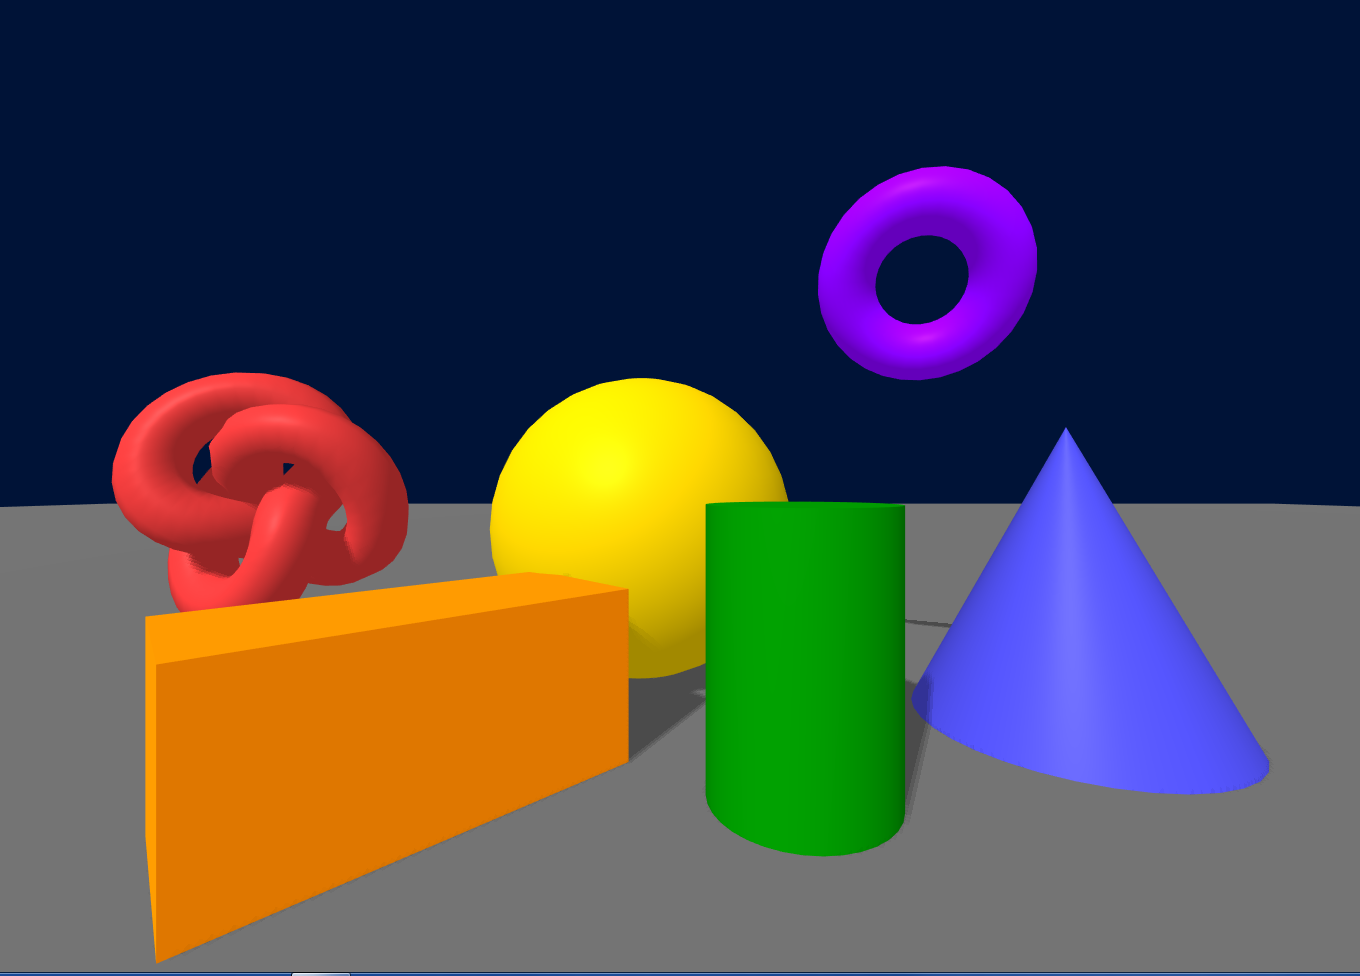
\includegraphics[width=1\textwidth]{img/Aframe.png}
    \caption{Algunos ejemplos de \textit{A-Frame}} 
    \label{fig:A-Frame}
\end{figure}

Esta creado a partir de \textit{HTML} de forma que sea sencillo de leer y comprender. De esta manera es accesible para crear una gran comunidad. \textit{A-Frame} sigue el patrón ECS(entidad-componente-sistema). Se trata de un patrón de desarrollo de juegos basado en el principio de composición sobre herencia. De esta manera, se otorga una mayor flexibilidad en la definición de entidades ya que cada objeto de la escena se corresponde con una entidad y cada entidad,a su vez, está compuesta por uno o más componentes que contienen datos y estado de la entidad. Por tanto, una entidad puede verse modificada en tiempo de ejecución si alguno de los componentes que agrega modifica sus datos

A-Frame, además de disponer primitivas como las mostradas, hace posible la creación de primitivas para poder elaborar escenas lo más completas posible. También se pueden incluir entidades más complejas a partir de modelos 3D en formatos como \textit{gltf}, \textit{obj} o \textit{collada} de los cuales se hablará en siguientes apartados.






% BLENDER %
\section{Blender}
\label{sec:blender}
\textit{Blender} es un programa libre dedicado al diseño y animación 3D. Mediante una interfaz gráfica permite diseñar objetos, personajes y escenas en tres dimensiones con muy diversas técnicas. Cada uno de los elementos creados pueden ser animados mediante \textit{keyframing} o animación por fotogramas clave. En su origen \textit{Blender} fue distribuido como una herramienta privada explotada por un estudio de animación, pero actualmente se encuentra bajo licencia \textit{GPL}\cite{bib:gpl}. 

    
\begin{figure}[ht]
    \centering
    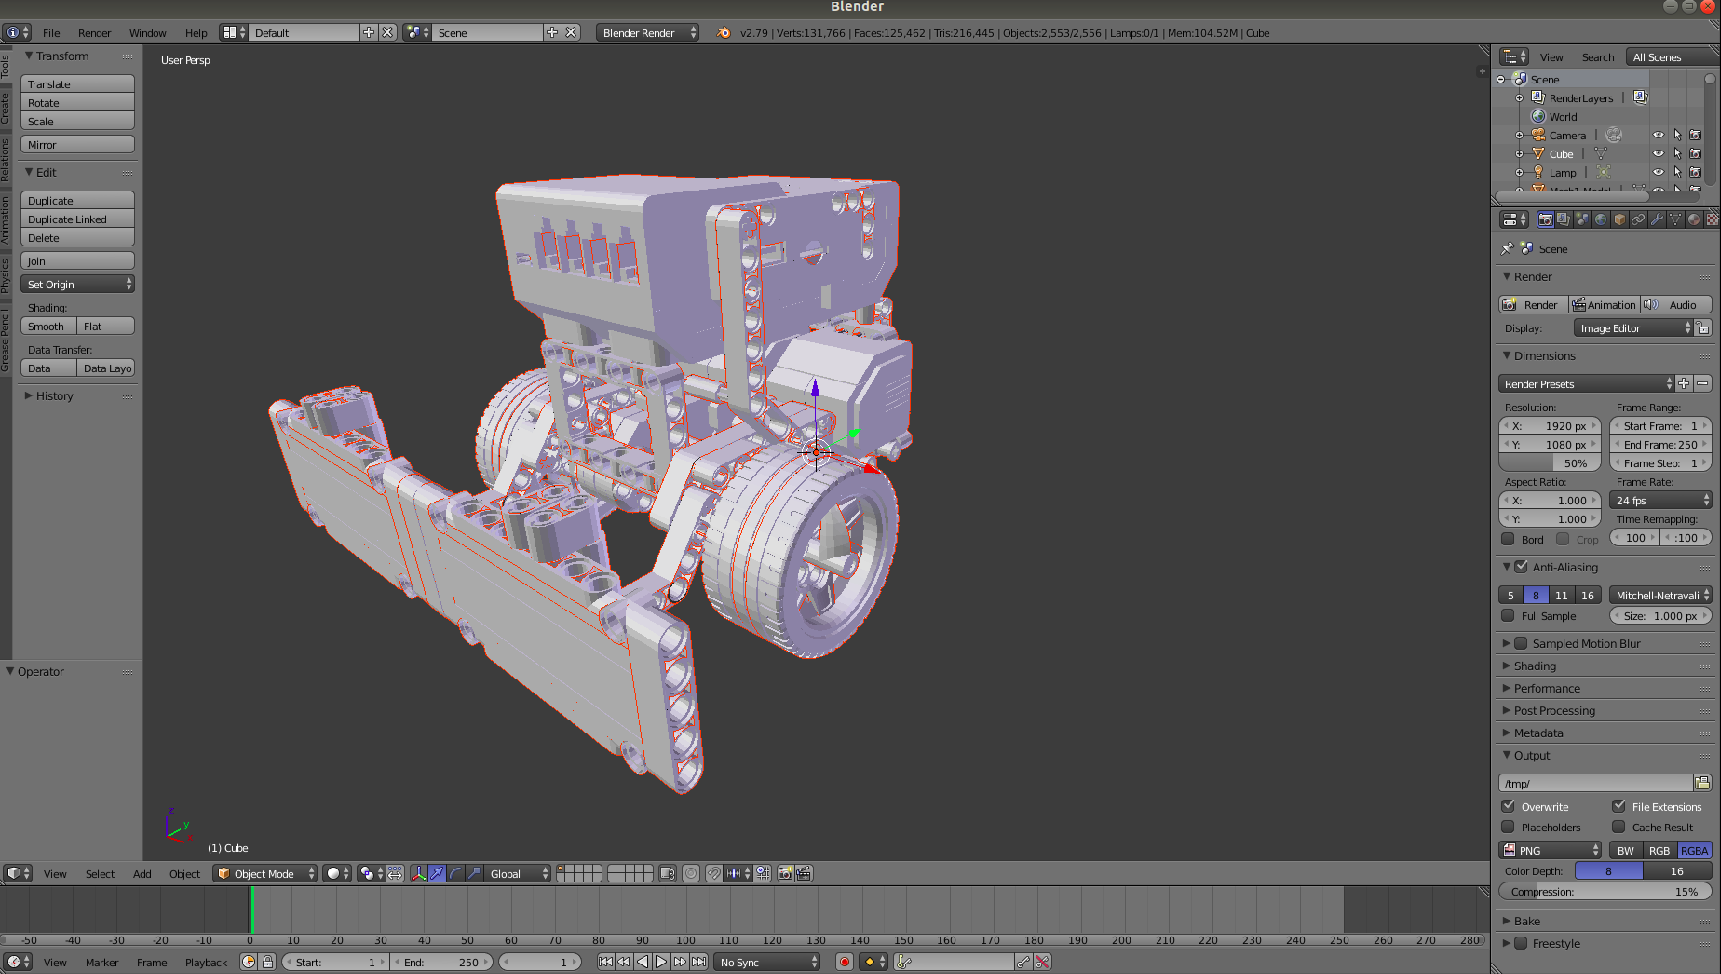
\includegraphics[width=1\textwidth]{img/primermodelo.png}
    \caption{Interfaz gráfica de \textit{Blender}} 
    \label{fig:blender}
\end{figure}

Existe un almacén web desde donde es posible descargarse una gran variedad de modelos y escenarios, además de desarrollar los propios. Una vez desarrollado el modelo o escenario, estos editores exportan el modelo o escenario en formato "gltf", que es el formato soportado por \textit{A-Frame} y estaría listo para insertarlo en el entorno simulado.\newline
Los escenarios y modelos generados por estos editores son creados mediante la intersección de líneas, generando los distintos tipos de objetos. Es posible adjuntar una textura o color a cada cara que forma el objeto. Además, el editor \textit{Blender}, al ser más complejo, permite la introducción de iluminación y trabajar con formas geométricas entres dimensiones directamente.\newline
Este es el programa que usaremos para crear los modelos del robot simulado.


% WEBSIM %
\section{Simulador WebSim}

\textit{Websim} es un simulador diseñado para enseñar conceptos básicos de tecnología e iniciar a niños en robótica y programación. 
\subsection{Diseño}
\label{subsec:design}
El simulador hace uso del entorno \textit{A-Frame} y su diseño permite conectar un editor de texto o un editor de bloques para  programar en \textit{JavaScript} o \textit{Blockly} y conectar este código con el robot simulado. También permite acoplar una aplicación externa al navegador a través de comunicaciones ICE. En la figura \ref{fig:websim} se puede ver el diseño de \textit{WebSim}.

Las principales funcionalidades del simulador son: 

\begin{itemize}
    \item Registrar los componentes principales para constituir un robot en \textit{A-Frame}, los cuales son \textit{followBody}, \textit{spectatorComponent} e \textit{intersectionHandler}. El primero se encarga de simular una cámara en el robot, el segundo maneja eventos de intersección de los láseres y el último permite anclar distintos elementos al robot simulado. 
    
    \item Ofrece una interfaz en diferentes lenguajes de programación \textit{JavaScript} para manejar el robot en el entorno simulado de \textit{A-Frame} llamada \textit{Hardware Abstraction Layer} (\textit{HAL API}). \textit{Websim} se encarga de enviar instrucciones al robot de manera sencilla sin necesidad de comunicarse con el motor de \textit{A-Frame}. 
    
    
    \item Permite manejar la ejecución de la simulación del robot. Es decir, permite lanzar o pausar la ejecución del robot e incluso reiniciar su posición para no tener que recargar la página en caso de querer probar distintos códigos con la misma simulación. Además este control del entorno evita que la variable \textit{myRobot} pierda el objeto instanciado porque el usuario cambie su valor.
    
\end{itemize}

Gracias a estas características, el simulador hace que los usuarios puedan programar de manera sencilla, ya que solo tienen que acceder a la información que ofrecen los sensores del robot y mandar órdenes sobre los actuadores del mismo. Es decir, solo  se tienen que encargar de programar la lógica del robot para resolver los ejercicios propuestos que se explicarán en próximos capítulos. 


\begin{figure}[H]
    \centering
    \includegraphics[width=1\textwidth]{img/websim.png}
    \caption{Interfaz gráfica de \textit{WebSim}} \label{fig:websim}
\end{figure}




\subsection{Drivers de sensores}
\label{subsec:driversSensores}
El robot consta de sensores simulados con \textit{A-Frame}. Los drivers permiten que el usuario, vía \textit{JavaScript}, pueda acceder a estos y obtener su información. En este entorno disponemos de los siguientes sensores: 

\begin{table}[H]
\caption{Métodos (HAL API) de los sensores del robot.}
\vspace{0.5cm}
\label{tab:tablaSensores}
\resizebox{\textwidth}{!}{%
\begin{tabular}{|c|c|c|ll}
\cline{1-3}
\textbf{Método} & \textbf{Descripción} & \textbf{Salida} &  &  \\ \cline{1-3}
.getDistance() & \begin{tabular}[c]{@{}c@{}}Devuelve la distancia entre el robot\\  y la intersección del raycaster en el centro\end{tabular} & number(metros) &  &  \\ \cline{1-3}
.getDistances() & \begin{tabular}[c]{@{}c@{}}Devuelve la distancia entre el robot y\\ la intersección con cada una de los raycaster\end{tabular} & list number(metros) &  &   \\ \cline{1-3}
.readIR(color) & \begin{tabular}[c]{@{}c@{}}Recorta la imagen, filtra y calcula el centro\\ del objeto con el color pasado como argumento\end{tabular} & number &  &  \\ \cline{1-3}
.getRotation() & \begin{tabular}[c]{@{}c@{}}Retorna un objeto con la orientación \\ del robot en los 3 ejes\end{tabular} & \begin{tabular}[c]{@{}c@{}}\{x:number,\\ y:number,\\ z:number\}\end{tabular} &  &  \\ \cline{1-3}
.getPosition() & Obtiene la posición del robot en la escena & \begin{tabular}[c]{@{}c@{}}\{x:number,\\ y:number,\\ z:number\}\end{tabular} &  &  \\ \cline{1-3}
.getImage() & Devuelve la imagen de la cámara del robot & cv.Mat() &  &  \\ \cline{1-3}
.getObjectColor(color) & \begin{tabular}[c]{@{}c@{}}Devuelve un objeto con la posición del elemento\\ detectado por la cámara del color pasado por parámetro\end{tabular} & \begin{tabular}[c]{@{}c@{}}\{center:{[}x.y{]},\\ area: int\}\end{tabular} &  &  \\ \cline{1-3}
.getObjectColorRGB(valorBajo,valorAlto) & \begin{tabular}[c]{@{}c@{}}Devuelve un objeto con la posición del elemento\\ detectado por la cámara con los valores pasados por parámetro\end{tabular} & \begin{tabular}[c]{@{}c@{}}\{center:{[}x.y{]},\\ area: int\}\end{tabular} &  &  \\ \cline{1-3}
\end{tabular}%
}
\end{table}

\subsection{Drivers de actuadores}
\label{subsec:driversMotores}

La función de los actuadores es otorgar movimiento al cuerpo del robot simulado en \textit{A-Frame}. Con los métodos creados, además, no es necesario mandarle órdenes constantemente, si no que es suficiente con mandar la instrucción una vez y el robot seguirá ejecutándola hasta que reciba una nueva.  


En la tabla \ref{tab:tablaMotores} se explican todas las funciones del \textit{HAL API} que hacen referencia a los actuadores.

\begin{table}[H]
  \begin{center}
    \caption{Métodos (HAL API) de los actuadores del robot.}
    \vspace{0.5cm}
    \label{tab:tablaMotores}
    \begin{tabular}{|c|c|} 
    \hline
      \textbf{Método} & \textbf{Descripción}\\
      \hline
.setV(integer) & \begin{tabular}[c]{@{}c@{}}Mueve hacia delante o atrás el robot.\\\end{tabular} \\ \hline
.setW(integer) & \begin{tabular}[c]{@{}c@{}}Hace girar al robot.\\\end{tabular} \\ \hline
.move(integer, integer) & \begin{tabular}[c]{@{}c@{}}Mueve el robot hacia delante/atrás y gira al mismo tiempo.\\ \end{tabular} \\ \hline
.getV() & \begin{tabular}[c]{@{}c@{}}Obtener la velocidad lineal configurada en el robot.\\ \end{tabular} \\ \hline
.getW() & \begin{tabular}[c]{@{}c@{}}Obtener la velocidad angular configurada en el robot.\\ \end{tabular} \\ \hline
    \end{tabular}
  \end{center}
\end{table}

Estos seran los \textit{drivers} que tenga que agregar a la funcionalidad tanto en el robot simulado, programado en \textit{JavaScript}  y el real que tendrá unos equivalentes en \textit{Python}.

\section{Django}

Django es un framework de código abierto escrito en Python, creado en 2005, el cual permite desarrollar un entorno web complejo de una forma rápida y estructurada. Actualmente es mantenido por Django Software Foundation y se encuentra en la versión 3.0 (Novapros, 2020).

Sigue una arquitectura MVC (Modelo – Vista - Controlador), como se observa en la figura(Holovaty y Kaplan-Moss, 2007).
\begin{itemize}
	\item \textit{Modelo}. Los modelos de datos creados están mapeados directamente a las tablas de la base de datos, permitiendo aislar el código de la aplicación de la base de datos.

	\item \textit{Vista}. Corresponde con la capa de presentación, y está basada en plantillas HTML.		
	\item \textit{Controlador (en Django llamado “views”)}. Responsable de seleccionar la plantilla a mostrar. Atiende a una petición y, según el mapeo de la URL, (Uniform Resource Locator) redirige a una vista u otra.
\end{itemize}
\begin{figure}[h!]
  \centering
    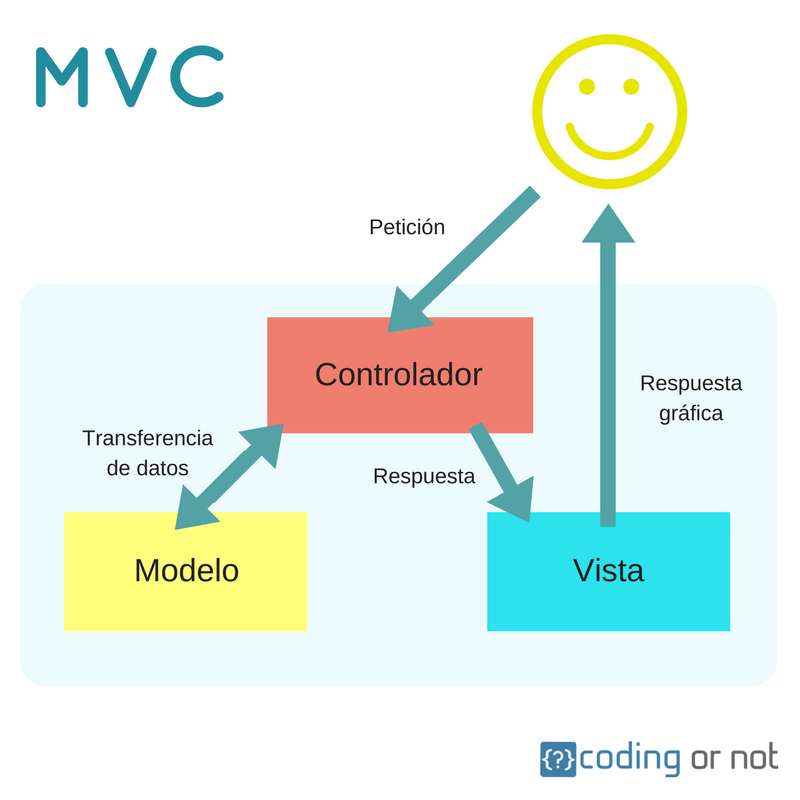
\includegraphics[width=0.6\textwidth]{img/mvc.png}
  \caption{Arquitectura Django}
  \label{Arquitectura Django}
\end{figure}
La meta fundamental de Django es facilitar la creación de sitios web complejos. Django pone énfasis en el re-uso, la conectividad y extensibilidad de componentes, el desarrollo rápido y el principio No te repitas (DRY, del inglés Don't Repeat Yourself). Python es usado en todas las partes del framework, incluso en configuraciones, archivos, y en los modelos de datos. 
Ofrece una serie de características bastante interesantes como es su excelente capa de seguridad (p ej. permite una protección contra los ataques maliciosos “Cross-site request forgery”), dispone de un sistema de administrador “por defecto,” sin necesidad de realizar ningún tipo de configuración. También proporciona una interfaz para el acceso a la base de datos, facilitando las consultas (Novapros, 2020).


\section{Flask}

Flask, lanzado en abril de 2010 es, junto con Django, uno de los framework webs más famosos escritos en Python.\newline
Está enfocado en proporcionar lo mínimo necesario para poner en funcionamiento una aplicación, por eso se le considera un framework “minimalista”. Por otro lado, no requiere de otras dependencias para realizar acciones básicas, de manera que la curva de aprendizaje para su comprensión es muy baja. Debido a su sencillez en la estructura, posee una velocidad mayor que Django y es bastante útil para iniciarse en el aprendizaje de desarrollo web, permitiendo crear servidores de una forma rápida. Debido a ello, Flask está orientado al sector servicios, los cuales implican muchas visitas y una carga grande de peticiones, y también para proyectos personalizados o sencillos (Rodríguez, 2019).
\begin{figure}[h!]
  \centering
    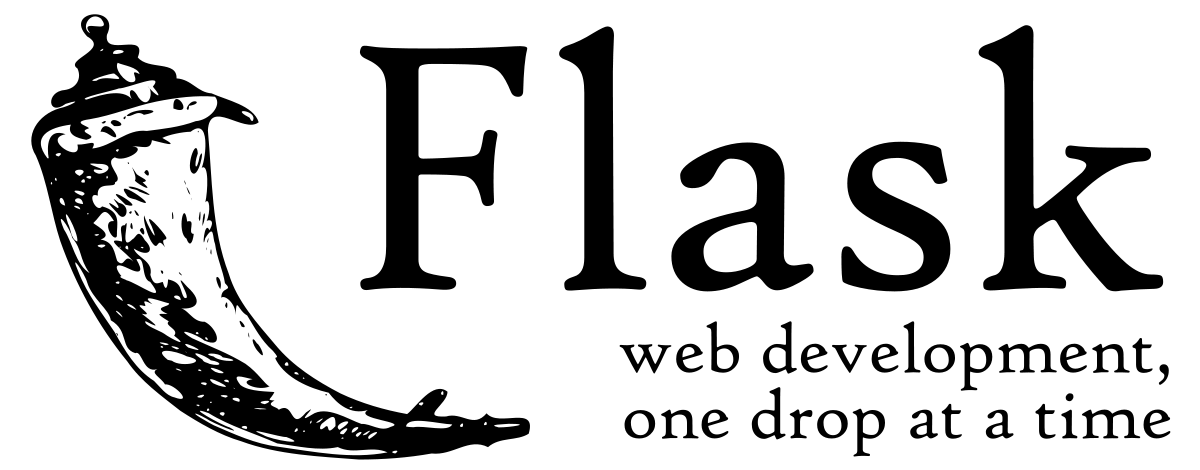
\includegraphics[width=0.4\textwidth]{img/flask.png}
  \caption{Logo Flask}
  \label{Flask}
\end{figure}